%*******************************************************************************
%*********************************** First Chapter *****************************
%*******************************************************************************

\chapter{Posture Generation, state of the Art, Introduction}


\nomenclature[z-PG]{PG}{Posture Generation}
\nomenclature[z-IK]{IK}{Inverse Kinematics}
\nomenclature[z-dof]{dof}{degrees of freedom}
\nomenclature[x-I]{$\mathbb{I}_n$}{Matrix identity of dimension $n$}


\graphicspath{{Chapter1/Figs/Vector/}{Chapter1/Figs/}}

\section{List of contributions}
\begin{itemize}
  \item Generalities, introduction
  \item Presentation of the existing methods
  \item From Inverse Kinematics to Generalized IK/posture Generation/pose estimation (addition of articular limits, forces, stability etc.
  \item Topology of the parametrization space (Free-flyer, q, f, other)
  \item Formulation as a non-linear constrained optimization problem
  \item Adrien \& Karim's formulations
  \item Formulation of several types of cost/constraints
  \begin{itemize}
    \item Contact with plane surface
    \item Collision avoidance
    \item Auto-Collision avoidance
    \item Static equilibrium: Newton/CoM projection
    \item Forces in friction cones
    \item Articular limits
    \item Torque limits
    \item Torque minimization
    \item Goal Posture
  \end{itemize}
  \item Reasons why it is not enough and why we needed a new PG
    \begin{itemize}
      \item Having an easier way to formulate problems
      \item Avoid having to de some gymnastic to remain on manifolds
      \item Automatic variable management
      \item Robustness
    \end{itemize}
  \item Utilization of posture generation in planning
\end{itemize}


%%%%%%%%%%%%%%%%%%%%%%%%%%
%  SECTION INTRODUCTION  %
%%%%%%%%%%%%%%%%%%%%%%%%%%

\section{Introduction}
\label{sec:introduction}

The ultimate goal of robotics is to make robots realize some tasks.
The tasks, as well as the robot used to fulfill them are various.
For example, it can be a robotic arm building a car in a factory, a surgeon robot operating on a human, a submarine robot exploring the wreckages of a ship, a humanoid robot exploring and fixing a destroyed nuclear plant.

\begin{figure}[ht]
  \centering
  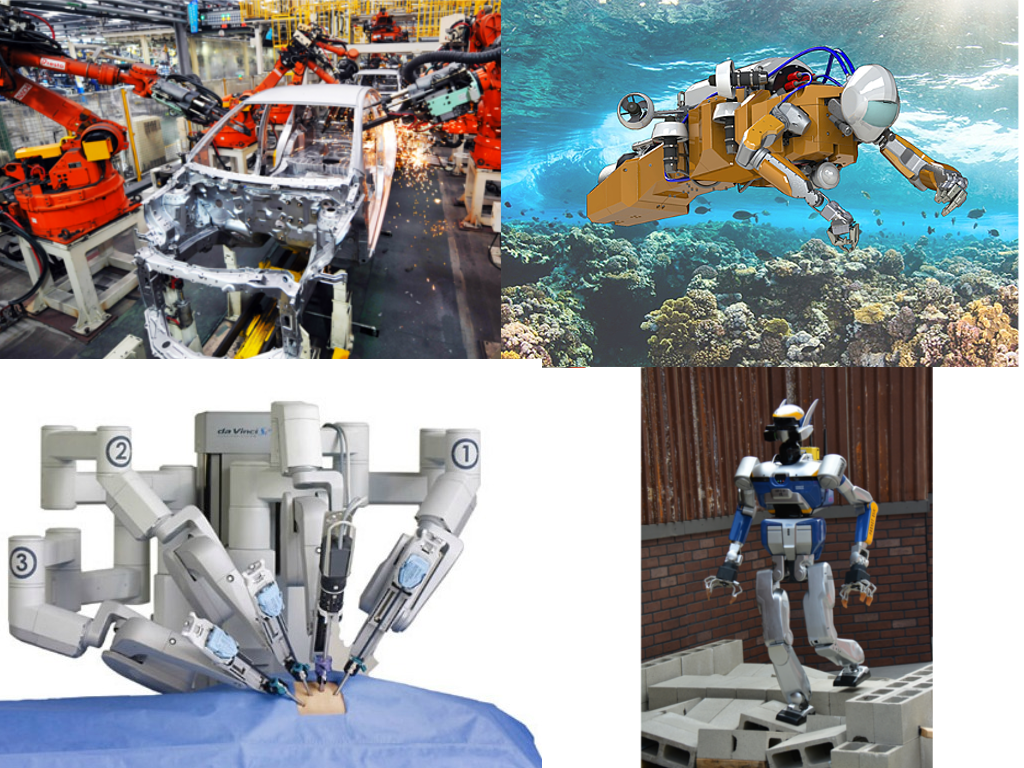
\includegraphics[width=0.9\textwidth]{various-tasks.png}
  \caption{Various robots doing various tasks}
  \label{fig:various}
\end{figure}

The DARPA Robotics Challenge has brought some light on the humanoid robots.
This competition brought together a large scope of robotics groups from universities, laboratories and private companies around a common goal: Make a robot succeed in several challenges without any human physical intervention.
The robots were expected to drive a car, open a door, climb stairs, cross debris, drill a hole in a wall, etc.
All those tasks can usually be broken down into sets of elementary tasks in human language.
Some typical examples of tasks for a robot can be "Put hand in contact with target", "Put foot on next step", "Avoid collision with that object", "Maintain stability" or "Look in that direction".
As is, those tasks do not mean anything for the robot.
A robot is made of a collection of bodies that are linked together by joints, that are actuated by motors.
A robots configuration consists of the position and orientation of its base body, and the configuration of each of its joints.
Satisfying a task requires that the joints of the robot reach a configuration for which the task is satisfied.
The action of satisfying a task comes down to moving from an initial configuration to a goal configuration, figuring out the trajectory to follow and actually following it are the jobs of the trajectory generation and the control of the robot.
Those are by themselves some complete fields of robotics, and they have one thing in common, they both need to be given an initial configuration, a final configuration and sometime some intermediate configurations.
Finding those configurations is the job of what we call the Posture Generation (PG), which is the main topic of this dissertation.
There are two types of robots. The fixed-base robots and the mobile robots.
The first type of robots have fixed basis, which mean that the area that they can reach is predefined by their geometry and are usually fully-actuated.
Which means that the robot has as many dof as actuators, Thus, for any joint configuration, a unique robots position is achieved.
On the contrary, mobile robots are under actuated, which means that the robot has more dof than actuators.
Each link of the robot is actuated, but the position of the basis of the robot is the result of the configuration of the joints and of the contacts that the robot makes with the environment.
A mobile robot's position depends on the location of its contacts with the environment.
For biped robots evolving on a flat surface, a footstep planner can be used to decide of the sequence of steps to take so the robot can walk to its goal.

Humanoid robots are expected to move and achieve tasks in ways similar to humans.

On flat surfaces, they can walk based on a cyclic motion and the locations of footsteps can be generated by a footstep planner using some simplified models to maintain the robots stability.
In cumbersome and unstructured environments, we humans move in a non-gaited acyclic way: we choose appropriate parts of our body to create contacts with the surrounding environment in order to support the motion of the remaining parts while avoiding obstacles.
A whole motion is a sequence of contact creations and releases.

Since we are biped, we mostly use our feet to move.
As the environment becomes more difficult to cross, hands may come into play together with feet to help with the motion.
Narrow passages may even require other parts of our body (knees, elbows, back...) to make contact in order to support the motion.

In the past few years, our team has dedicated considerable efforts in proposing a general multi-contact motion planner to solve such cases of non-gaited acyclic planning.
Given a humanoid robot, an environment, a start and a final desired postures, the planner generates a sequence of contact stances allowing any part of the humanoid to make contact with any part of the environment to achieve motion towards the goal.
The planner's role is to grow a tree of contact stances iteratively, from a given posture, it tries to removes one of its contacts or to add a new one.
The tree grows, following some heuristics until the solution is reached.
A typical experiment with a HRP-2 robot achieving such an acyclic motion is presented in~\cite{escande:iser:2008}, and the planner is thoroughly described in~\cite{escande:ras:2013}.
Extensions of this multi-contact planner to multi-agent robots and objects gathering locomotion and manipulation are presented in~\cite{bouyarmane:ar:2012}, and preliminary validations with some DARPA challenge scenarios, such as climbing a ladder, ingress/egress a utility car or crossing through a relatively constrained pathway are presented in~\cite{bouyarmane:humanoids:2012}.
\cite{hauser:issr:2007} presents a different approach to multi-contact planning based on probabilistic roadmap and random sampling of the configuration space.
Another way of planning a multi-contact scenario, which is actually the most popular, is to do it by hand, the user chooses iteratively which contacts to add and remove until the goal is reached.

Planning the sequence of contacts to achieve is a necessary step in devising a motion for a robot.
Once the key stances of the motion have been identified by the planner, they can be used by the controller or the trajectory planner and finally the motion can be achieved by the robot.

All the aforementioned planning method rely on the fact that we have a tool to decide if a proposed set of contact is feasible or not for the robot.
The tool used for finding a robot configuration that satisfies a set of constraints like the geometric constraints of contact is called a "Posture Generator" (PG) and the development of that tool is the main topic of this dissertation.

The mission of a posture generator is, for a poly articulated system, to find a configuration so that the system satisfies a set of constraints.
For simple systems, with simple constraints, like a 6 dof robotic arm having to reach a point with its end effector, some closed-form expressions can usually be devised.
But computing robot configuration to meet the requirements of a given set of tasks, within a viable state, is a recurrent problem whose complexity grows with that of the robot.
When the robotic problem studied becomes too complex for closed-form formulas, it is formulated as a non-linear optimization program and solved using state of the art optimization algorithms.

Because it is a key element for many robotics application, the posture generator is a very important element of any robotics framework.
It needs to be efficient at finding a solution when one exists and at figuring when a problem is not feasible.
The speed of generating a multi-contact sequence is directly related to the quality of the posture generator.

If we consider a problem of posture generation on a mobile robot with $n$ joints, the configuration space of the joints of the robot is $\mathbb{R}^n$ and the configuration space of the position and orientation of its base body is $SE(3) = \mathbb{R}^3\times SO(3)$.
Thus, the variable that describes the configuration of the robot in the optimization problem lives in $\mathbb{R}^3\times SO(3) \times \mathbb{R}^n$.
$SO(3)$ is by nature a non-Euclidean manifold, it cannot be parameterized on an open subset of Euclidean space without having to deal with problems of gimbal lock.
The gimbal lock is a singularity that happens when parameterizing $SO(3)$ on $\mathbb{R}^3$, with Euler angles, for example, and when two axis of rotation become aligned, in that situation, 2 elements of the parameterization correspond to the same rotation.
Thus, one degree of freedom is lost.
Note that this singularity can block the optimization algorithm and that it is only due to the choice of parameterization, it is not intrinsic to the manifold $SO(3)$.
It is possible to parameterize $SO(3)$ without having to face singularities by parameterizing it over another non-Euclidean manifold.
The most common ones being the unit quaternion space and the $3\times 3$ rotation matrix.
Most of the solvers available make the assumption that the search space is Euclidean, which makes is complicated to use quaternion or rotation matrix efficiently.
To put it simply, for the unit quaternion parameterization, a variable on $SO(3)$ is represented by 4 parameters, the coefficients of the quaternion and an equality constraint needs to be added to the optimization problem to ensure that the quaternion is of norm 1, $\{q\in\mathbb{R}^4:||q||=1\}$.
Similarly, if a variable is parameterized by a rotation matrix, then the variable $M$ has 9 parameters and several constraints need to be added to the problem so that M is symmetric, positive definite and its determinant is 1 $\{M\in\mathbb{R}^{3\times 3}:M^TM = \mathbb{I}_3\  \&\ \det (M) = 1\}$.
Similar issues can be found with the parameterization of other non-Euclidean manifold, like $S2$ for example.

There exists some methods and algorithms to solve optimization problems on non-Euclidean manifolds with no substantial extra cost and guaranteeing a good coverage of the manifolds without facing parameterization singularities and with the minimal number of parameters.
Though to our knowledge, they are focused on non-constrained optimization.
One of the particularity in our approach of posture generation is that we develop, extend and use one such optimization algorithm on non-Euclidean manifolds to solve robotics problems.

\subsection{Posture Generation}
\label{sub:posture_generation}

Posture Generalization can be viewed as, and is sometimes called, Generalized Inverse Kinematics.
The Inverse Kinematics problem consists in finding the joint configuration for an articulated to complete a given task.
It is, by definition purely kinematics, it has no regards for stability, or other physics related constraints.
The IK problem has been widely studied and used in the fields of robotics, computer graphics, computer games and animation.
For the simplest cases, with robotic arms that have less than 7 degrees of freedom, a closed-form solution can be found.
But for more complicated cases, optimization methods are usually used.
\cite{aristidou2009} presents a review of existing techniques to solve inverse kinematics and one can see that the optimization approaches to that problem are various: Inverse Jacobian, Newton method, Sequential Monte Carlo and Heuristic approaches. It also presents a novel geometric iterative heuristic approach.

The Generalized Inverse Kinematics refers to a problem similar to the Inverse Kinematics in the sense that it searches a joint configuration for an articulated figure to complete a task under several other constraints like ensuring the stability of the structure, respecting its joint limits, avoiding collision with the environment or with itself.

\subsection{Optimization}
\label{sub:optimization}

\section{Problem Definition}
\label{sec:problem_definition}

We consider a robot $\mathit{R}$ with $n$ degrees of freedom (dof), its joint configuration can be described by a point on

\section{From Inverse Kinematics to Posture Generation}
\label{sec:from_inverse_kinematics_to_posture_generation}

The problem of finding a configuration of a poly articulated system to satisfy some geometric constraints has been widely studied for decades under the name of Inverse Kinematics (IK).
IK is an important tool in many fields like robotics, computer graphics and animation.




%%%%%%%%%%%%%%%%%%%%%%%%%
%  SECTION FORMULATION  %
%%%%%%%%%%%%%%%%%%%%%%%%%

\section{Formulation}

Here we present the basic formulation of a PG problem.

The free-flyer, the articular space and the forces being the usual variables.

Presentation of all the constraints and their formulation
\begin{itemize}
  \item Joint limits
  \item Auto-collision
  \item Collisions with environment
  \item Contacts with environment
  \item Stability
  \item Torque limits
\end{itemize}

